\chapter{Interferometry, Calibration \& Polarimetry}
\label{chapter:interferometry}

In this Chapter I wished to build a formalism around wide-field, polarized interferometric measurements that could be used throughout this work. Many traditional assumptions used in radio interferometry are broken in the case of the wide-field, fully-polarized, drift-scanning measurements native to interferometric EoR observations. In Section~\ref{sec:interferometry_vis}, I derive the equation describing the fundamental observable for an interferometer, called a ``visibility". Section~\ref{sec:interferometry_cal}, I describe calibration techniques relevant to this work and in Section~\ref{sec:interferometry_pol} I review some of the implications of the previous two sections for polarized measurements.

For a comprehensive review of interferometry from a more traditional perspective, see \cite{TMS}.

\section{The Visibility Equation}
\label{sec:interferometry_vis}

A radio interferometer (a term used interchangeably with ``interferometric array" for radio observations) is an ensemble of receiving elements, where each element's measurement is correlated with every other element's. The simplest case is a two-element interferometer, which we will focus on below. We assume that the elements are coplanar and identical.

\subsection{The Classical Visibility Equation}

Consider two receiving elements $i$ and $j$, separated by baseline vector $\vec{b}$. Suppose a plane wave of wavelength $\lambda$ is incident upon these elements, with direction of propagation $-\hat{s}$. The geometry of this interferometer is illustrated in Figure~\ref{fig:interferometry_2element}.

\begin{figure}
\centering
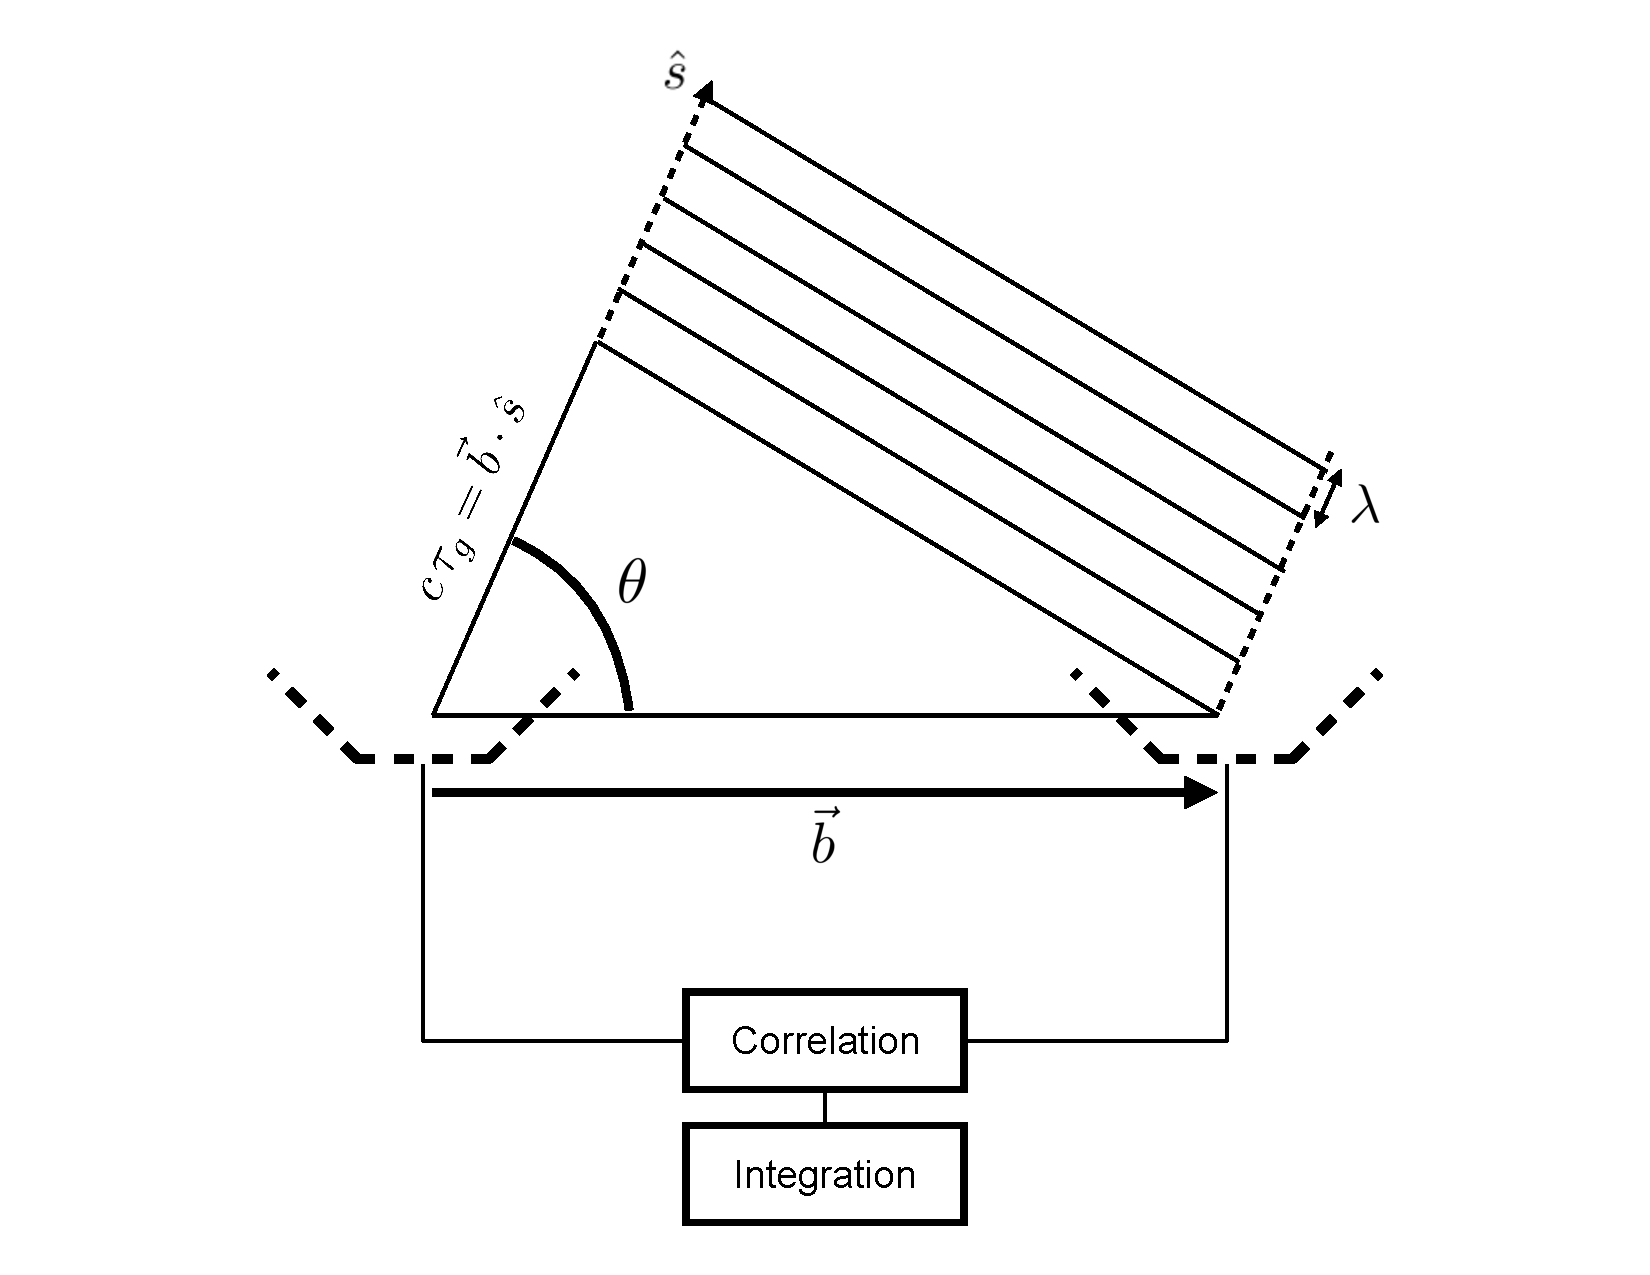
\includegraphics[width=0.9\textwidth]{chapters/interferometry/figures/visibility_explanation.pdf}
\caption{The geometry of a two-element interferometer, with a plane wave incident from direction $\hat{s}$.}
\label{fig:interferometry_2element}
\end{figure}

We can define the electromagnetic wave to have a frequency dependent phase, such that the electric field measured by element $i$ at time $t$ is

\begin{equation}
E_i = E_0 e^{-2\pi i \nu t}.
\label{eq:Ei}
\end{equation}

The time difference between the arrival at $i$ and $j$ is called the ``geometrical delay", $\tau_g$:

\begin{equation}
\tau_g = \frac{\vec{b}\cdot\hat{s}}{c},
\end{equation}
and the electric field measured by element $j$ is

\begin{equation}
E_j = E_0 e^{-2\pi i \nu (t+\tau_g)}.
\end{equation}

An interferometer is an instrument which correlates these electric fields together, integrating their product over some coherent time-scale. This correlation grants:

\begin{equation}
\langle E_i E_j^* \rangle 
= \lim_{T\rightarrow\inf}\frac{1}{2T}\int^T_{-T} E_i(t) E_j(t) {\rm d}t
= | E_0 |^2 e^{-2\pi i \nu \tau_g}
\end{equation}
where $e^{-2\pi i \nu \tau_g} = e^{-2\pi i \nu \vec{b}_{ij}\cdot\hat{s}/c}$ is known as the ``fringe" term, due to its sinusoidal nature. We can generalize this relationship to include more than a single plane wave from direction $\hat{s}$. Many plane waves, from all directions, can be incident upon the interferometer at a given time and frequency. We can represent the power distribution on the sky as $S(\Omega)$, where $S(\Omega)$. However, no instrument is equally sensitive to radiation from every direction $\hat{s} \in \Omega$. Instead, an instrument has some sensitivity pattern -- a \textit{beam pattern} -- that tapers the power distribution on the sky into an ``observed sky",  $S'(\Omega) = A(\Omega)S(\Omega)$. 

These generalizations lead to the classical visibility equation:

\begin{equation}
V_{ij}(\nu) = \int A(\Omega, \nu) S(\Omega, \nu) e^{-2\pi i \nu \vec{b}_{ij}\cdot\hat{s}/c} {\rm d}\Omega
\label{eq:classical_visibility}
\end{equation}
for a ``visibility" -- the fundamental interferometric observable -- $V_{ij}$ as a function of frequency.

If we choose to represent the source direction in terms of directional cosines $\ell$ and $m$, and represent the baseline vector in units of wavelengths, $\vec{b}_{ij}/\lambda=(u,v,w)$, we can perform a change of variables in Equation~\ref{eq:classical_visibility} to give

\begin{equation}
V_{ij}(u,v) = \int\int A(\ell, m)S(\ell, m) e^{-2\pi i (u\ell + vm + w\sqrt{1 - \ell^2 - m^2})} \frac{ {\rm d}\ell {\rm d}m }{\sqrt{1 - \ell^2 - m^2}}.
\label{eq:vis_def_widefield}
\end{equation}

This relationship is often simplified by assuming only a small area of the sky is under observation -- that is, that $A(\ell,m)$ falls-off steeply from zenith -- and therefore $\ell^2$ and $m^2$ are small. This grants

\begin{equation}
V_{ij}(u,v) \approx e^{-2\pi i w} \int\int A(\ell, m)S(\ell, m) e^{-2\pi i (u\ell + vm)} {\rm d}\ell {\rm d}m,
\label{eq:vis_dev_narrowfield}
\end{equation}
which plainly casts $V(u,v)$ as the Fourier transform of the observed sky if $w$ is small: that is, the array is co-planar and no appreciable curvature of the sky is probed. Modern low frequency interferometers used in this work greatly violate this approximation, the consequences of which I will discuss in the proceeding sections.

Even though it is often violated, the Fourier relationship shown in Equation~\ref{eq:vis_dev_narrowfield} is an extremely useful one to work with when translating between visibilities and images. Images can be created by inverse Fourier transforming all of the visibilities measured by an array. Following Equation~\ref{eq:vis_def_widefield}, a reconstructed image $\tilde{S}(\ell, m)$ is given by

\begin{equation}
\frac{A(\ell, m)\tilde{S}(\ell, m)}{\sqrt{1 - \ell^2 - m^2}} = \int\int \Xi(u, v) V(u,v) e^{2\pi i \nu (u\ell + vm)} {\rm d}u {\rm d}v.
\label{eq:image_estimate}
\end{equation}

In Equation~\ref{eq:image_estimate}, we see that the reconstructed image $\tilde{S}(\ell, m)$ is attenuated by the beam response $A(\ell, m)/\sqrt{1 - \ell^2 - m^2}$. The function $\Xi(u, v)$ defines the sampling of the $u,\,v$ - plane. It is equal to 1 at the points sampled by the interferometer (baselines of length and direction defined by the vector  $\vec{b} = (u,v)$ exist in the array) and 0 elsewhere.

The effect of the sampling function $\Xi(u, v)$ is that the true sky $S(\ell,m)$ can never be completely reconstructed, since it is impossible to build an interferometer that samples every $u,v$ mode. The true sky is convolved with the Fourier transform of $\Xi(u, v)$, which astronomers refer to as the ``dirty beam". $\Xi(u, v)$ contains zeros, so a complete deconvolution of $\tilde{S}(\ell, m)$ is impossible.

We now note that an important aspect of light has been absent throughout the derivations above: the polarization state of the radio wave that induces the electric field in Equation~\ref{eq:Ei}. Interferometers are typically constructed with two feeds, sensitive to polarization states of an incident radio wave along two separate axes. In the case of all of the instruments used in this work (see Chapter~\ref{chapter:instruments}), an antenna $i$ had two dipole feeds perpendicular to one another. These were along the North-South direction (`n') and the East-West direction (`e'). We can attempt to generalize Equation~\ref{eq:classical_visibility} to include polarization, setting antenna $i$ to have orientation $p$ and antenna $j$ to have orientation $q$, $p,q\in(e,n)$:

\begin{equation}
V^{pq}_{ij} = \int A_{pq}(\Omega, \nu) S_{pq}(\Omega, \nu) e^{-2\pi i \nu \vec{b}_{ij}\cdot\hat{s}/c} {\rm d}\Omega.
\end{equation} 
However, two aspects of this equation are unsatisfactory. As explored in Chapter~\ref{chapter:astropol}, the polarized sky is defined with the four Stokes parameters; an ``$S_{pq}$" polarized sky does not exist. Likewise, a dipole is not purely sensitive to a single vector orientation from the sky, but probes a wide range of angles\footnote{In the case of the PAPER instrument, described in the next Chapter, the dipole feeds probed the entire hemisphere of the sky.}. Therefore a $A_{pq}$ polarized beam is ill-defined. These shortcomings lead us to rewrite the visibility equation, cohesively including polarization from the outset.  

\subsection{The Measurement Equation}

The Radio Interferometric Measurement Equation (RIME) provides an extremely useful framework for describing wide-field polarized observations. Formulated by \cite{HBS.1.96}, it was re-introduced to the radio astronomy community through a series of papers by O.~L. Smirnov \citep{Smirnov.11, Smirnov.11.2, Smirnov.11.3, Smirnov.11.4}. In this section I review the portions of his work most relevant to this thesis, and defer the reader to the series for a useful and thorough walk-through of wide-field radio interferometry.

% building the [classical] visibility equation in the unpolarized case
% pointing vs drift-scanning
% wide field effects
% rebuilding the visibility equation for widefield, polarized instruments
% Stokes visibilities -- previous chapter defines Stokes Parameters -- discuss pseudo-ness

\section{Calibration Techniques}
\label{sec:interferometry_cal}

% basics of calibration for drift-scanning interferometers
% redundant calibration theory (more in polcal chapter)
% redundant vs imaging configurations
% CLEAN: Hogbom, 1D-CLEAN [NEEDS DELAY] (Parsons & Backer), linCLEAN

\section{Instrumental Polarization}
\label{sec:interferometry_pol}

%%% Instrumental polarization:
% explore the matrix-formalized visibility equation
% DI leakage (calibration errors)
% DD leakage (cannot calibrate away -- must model)